\documentclass[handout]{beamer}

%FIXME: Eigentlich hasse ich einpoppende Folienteile, aber ich verwende sie dann doch sehr häufig... Generell und immer wieder den Folienaufbau neu überdenken.

\usetheme{Siegen}
\usecolortheme{LILA} 


% Im Beamertheme Siegen ist festgelegt:
% 1. Innertheme: Alles was auf der weißen Fläche in der Mitte passiert (Blocks, enumerate,...)
% 2. Outertheme: Alles was in den Kopf und Fußzeilen passiert.
% 3. Colortheme: Alles was mit Farben zu tun hat.

% Variationen
% Mit "\useinnertheme{xxx}", "\useoutertheme{xxx}" und "\usecolortheme{xxx}" können die einzelnen Teile unabhängig voneinander verändert werden.

% 1. Das Innertheme kann natürlich uneingeschränkt verändert werden, ohne vom Corporate design abzuweichen. (Möglichkeiten siehe beameruserguide.pdf) 

% 2. Das Outertheme ist für das Corporate design verantwortlich. Theoretisch muss die Fußzeile nur blau sein, was darin steht ist jedem selbst überlassen. Ich habe hier Referent (Uni) und einen Folienzähler verortet. Wenn das geändert werden soll, muss man direkt in den Quellcode von "beamerouterthemecdSiegen.sty" eingreifen.  

% 3. Colortheme: 
% a) Colortheme "GELB" (Uni-blau und Uni-Sekundärfarbe-gelb/organge) 
%    [default-Einstellung] 
% b) Colortheme "LILA" (Uni-blau und Fakultäts-lila)


\usepackage{graphicx}
\usepackage[utf8]{inputenc}
\usepackage[ngerman]{babel}
\usepackage{amsmath, amssymb, amsfonts, amsthm}
\usepackage{tikz}
\usepackage{siunitx}
\usepackage{graphicx}
\usepackage{pdfpages}

%\usepackage{feynmp-auto}
%\usepackage{feynmp}
\DeclareGraphicsRule{*}{mps}{*}{}
\unitlength = 1mm


\hypersetup{pdfborderstyle={/S/U/W 0}} % das brauche ich, damit meine Tex-Version nicht komische Verlinkungen zwischen den Sektions macht -- ihr braucht das vielleicht nicht, aber es schadet auch nicht.
% komische Verlinkungen?


% Folgende Zeilen definieren meine Zitat-Umgebung:
\newcommand{\Untertitel}
  {\begin{flushright}\tiny \rm\textsc{\Quelle}\end{flushright}}

\newenvironment<>{zitat}[1]%
{\begin{beamerboxesrounded}[upper=white, lower=white, shadow=true]{}%
 \newcommand{\Quelle}{#1}}%
{\Untertitel\end{beamerboxesrounded}}

\newcommand{\Wendy}[1]{\textcolor{red}{#1}}

\title{Identität und Passwörter}
\subtitle{Crypto Workshop}
\author[]{Jörg Germeroth / Tobias Becker}
\institute[Uni Siegen]{Crypto-Initiative \\ Universität Siegen}
\date{\today}

\begin{document}
\begin{frame}

  \maketitle  

\end{frame}

\begin{frame}{Worüber wollen wir gleich sprechen?}
    \tableofcontents[pausesections]
\end{frame}


\section{Typen von Identitäten}
\subsection{Wer bin ich?}
\begin{frame}{Wer bin Ich?}
Es gibt drei Antworten auf diese Frage:\\
\begin{itemize}
\item Ich bin Tobias Becker\\
Einwohnermeldeamt
\item Ich bin shguro\\
Internet Forum
\item Ich bin anonymous\\
Joodel
\end{itemize}
\end{frame}
\subsection{Pseudonym genüber Anonymität}
\begin{frame}{Pseudonym genüber Anonymität}
\begin{alertblock}{Pseudonym}
Ein Pseudonym ist quasi eine zweite Identiät welche normal nicht auf die echte Identiät zurückschießen lässt, jedoch eine Zuordnung einer Identität.\\

\end{alertblock}
\begin{alertblock}{Anonym}
Anonym zu sein bedeutet keine zuordnebare Identität zu haben\\
\end{alertblock}
\end{frame}
\section{Identität -- Wer bin ich?}% \Wendy{- Ich im Internet; -Wer bin ich im Internet}
\subsection{Das Ich im Internet? }%\Wendy{Wer bin ich?}}

\begin{frame}{Wer bin ich im Internet} %\Wendy{Ich im Internet (Handlungen so mit drin)}
    \begin{itemize}
        \item auf Facebook
        \item bei eBay
        \item bei Wordpress
        \item auf Twitter
        \item bei Reddit
        \item aber auch Online--Banking
        \item usw.
    \end{itemize}
\end{frame}

%FIXME Formulierung?oogle
\begin{frame}{Wer bin ich im Internet}
    %Da steckt Geld, das persönliche Leben und teilweise sogar die Karriere drin.
    Das bedeutet: Mein Geld, mein persönliches Leben und meine Karriere (evtl. Privatleben)!
\end{frame}

% Pseudo--/Anonymitäts Einschub (Advanced Thema)
%\begin{frame}{}
%    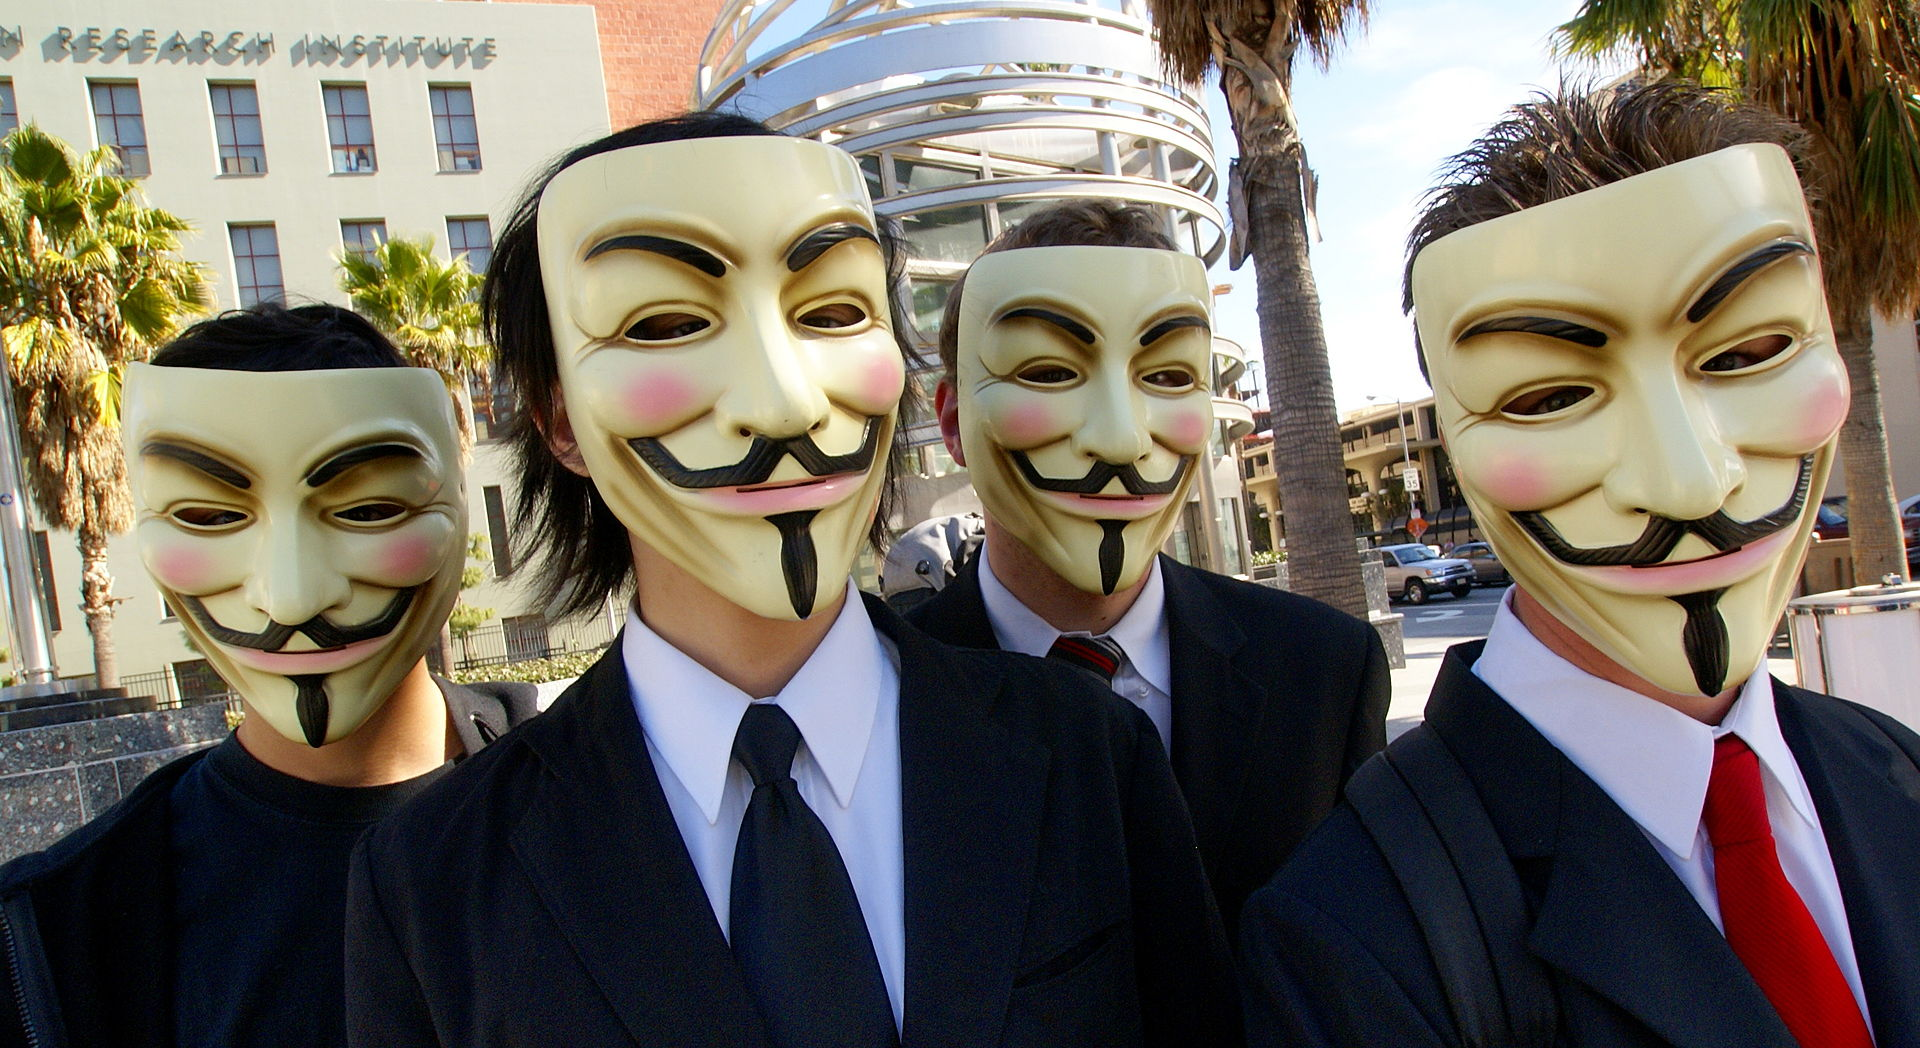
\includegraphics[width=\textwidth]{Bilder/Anonymous.jpg}
%\end{frame}

\section{Passwörter}
\subsection{Warum sind Passwörter so wichtig?}

%FIXME Die Folie gefällt mir noch nicht...
\begin{frame}{Warum sind Passwörter so wichtig?}
    \begin{alertblock}{Ganz einfach:}
        Weil sie meist die einzige Möglichkeit sind unsere Internet--Identitäten zu schützen!
    \end{alertblock}
    \pause
    %Sie sind das Hindernis, das die \glqq{}bösen Jungs\grqq{} davon abhält unsere Identität zu missbrauchen.
    %Nur s
    Sie halten die \glqq{}bösen Jungs\grqq{} davon ab, unsere Identität zu missbrauchen.
\end{frame}

\subsection{Wie sehen \glqq{}gute\grqq{} Passwörter aus?}

\begin{frame}{Wie sehen \glqq{}gute\grqq{} Passwörter aus?}
    \begin{block}{Passwortpolicy der Uni--Siegen}
        Das Passwort muss folgende Voraussetzungen erfüllen:
        \begin{itemize}
            \item Der Benutzername darf nicht Teil des Passwortes sein.
            \item Das Kennwort muss die Mindestlänge von 8 Zeichen haben.
            \item Das Kennwort muss Zeichen aus mindestens 3 der folgenden Kategorien enthalten
            \begin{itemize}
                \item Kleinbuchstaben,
                \item Großbuchstaben,
                \item Ziffern oder
                \item Sonderzeichen.
            \end{itemize}
            \item Die Verwendung von Umlauten oder ß wird nicht empfohlen.
        \end{itemize}
    \end{block}
\end{frame}

\begin{frame}{}
    \begin{center}
        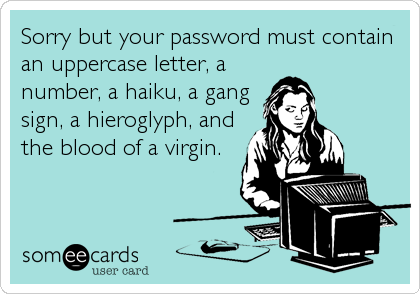
\includegraphics[width=0.8\textwidth]{Bilder/bloodvirgin.png}
    \end{center}
\end{frame}

%FIXME: Eigentlich ist diese Folie viel zu voll... Mir fällt aber keine bessere Darstellungsweise ein.
% Bild? Diagramm? 
% Jörg: Hmm, könnte funktionieren, kommt auf die Darstellung an. Die momentanen find ich gerade nicht ganz super, logarythmischer Graph für Fak1-Leute...
\begin{frame}{Warum so kompliziert?}
    \begin{block}{Einige Beispiele: so lange braucht es alle Kombinationen durch zu probieren}
        \begin{itemize}%[<+->]
            \item Alle Zeichen (96), Passwortlänge: 4
                \\\vspace{-0.45ex}\quad weniger als 1 Sekunde
            \item Alle Zeichen (96), Passwortlänge: 6
                \\\vspace{-0.45ex}\quad 13 Minuten
            \item Groß-- und Kleinbuchstaben + Ziffern, Passwortlänge: 8
                \\\vspace{-0.45ex}\quad 3 Tage
            \item Alle Zeichen (96), Passwortlänge: 8
                \\\vspace{-0.45ex}\quad 84 Tage
            \item Alle Zeichen (96), Passwortlänge: 12
                \\\vspace{-0.45ex}\quad 19 Millionen Jahre
        \end{itemize}
    \end{block}
    \pause
    Diese Zahlen gelten für einen normalen Standard--PC aus dem Jahr 2011.
    %Ein solcher PC schafft 1 Milliarde Schlüsseln pro Sekunde.
    \\\vfill
    \begin{center}\scriptsize{(Quelle: https://de.wikipedia.org/wiki/Passwort\#Ausprobieren\_von\_Passwörtern)}\end{center}
\end{frame}
%Zahlen als lin und log plot eingefügt!
%\begin{frame}{Graphisch:}
%    \begin{center}
%        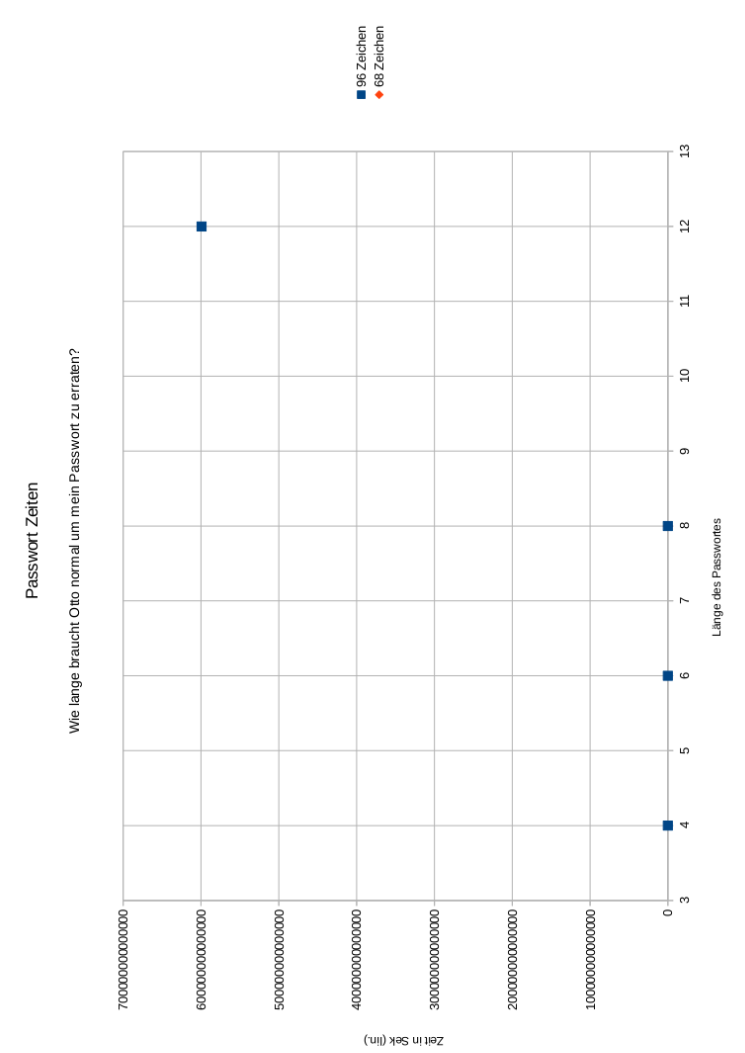
\includegraphics[width=0.55\textwidth, angle=270]{Bilder/passwortZeitLin.png}
%    \end{center}
%\end{frame}
%\begin{frame}{Graphisch:}
%    \begin{center}
%        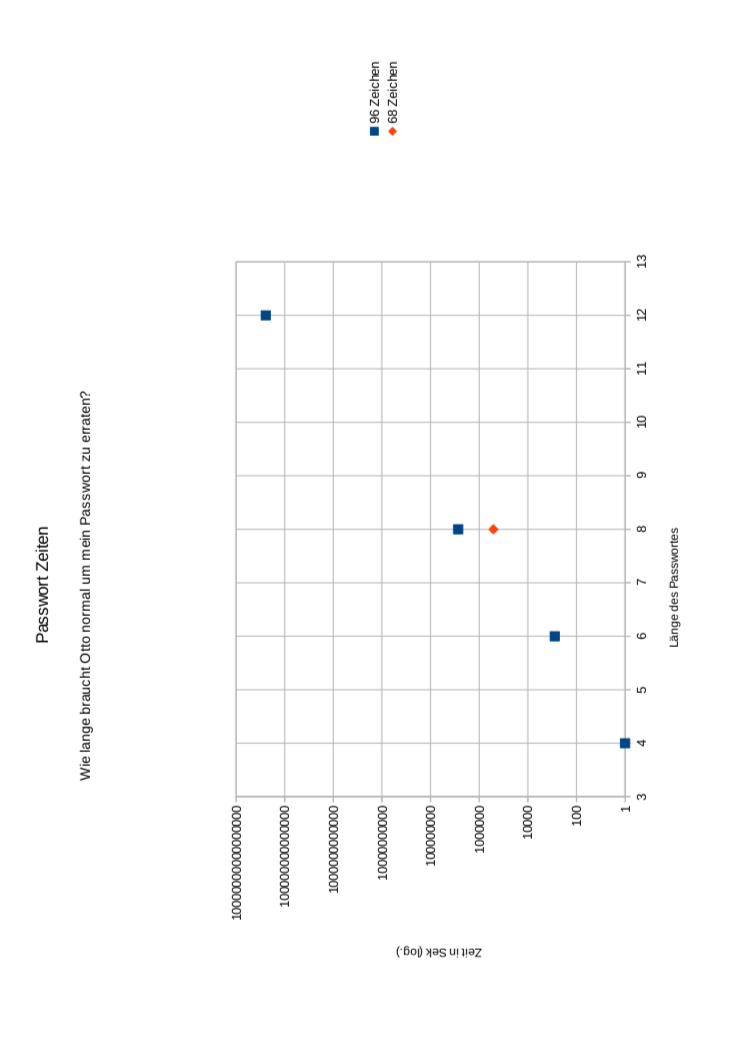
\includegraphics[width=0.6\textwidth, angle=270]{Bilder/passwortZeitLog.png}
%    \end{center}
%\end{frame}


\subsection{%Und wie kann ich mir den Mist merken? \Wendy{
Wie soll ich mir das alles merken?}% - Und wie kann ich mir das Chaos merken?}}
\begin{frame}{Aber das ist so schwer zu merken...}
    \begin{itemize}[<+->]
        \item pauken, pauken, pauken...
        \item Eselsbrücken
        \item ...aufschreiben
        \begin{itemize}
            \item auch wenn viele davon abraten
            \item oder es sogar verbieten
            \item aber: sicher aufschreiben; sicher verwahren!
        \end{itemize}
        \item Hilfsprogramme, die sich die Passwörter für einen merken
        \begin{itemize}
            \item KeePassX (Windows, OS X, Linux, Open Source)
            \item 1Password (Windows, OS X, Android, iOS, nur gegen Geld)
        \end{itemize}
    \end{itemize}
\end{frame}
% Benni: CT Passwort Karte eingefügt, ist vermutlich übersichtlicher, als sie an die wand zu malen!
% Jörg: Tafelbild hat nur den Vorteil, das es die Folien nicht überlädt, bzw. vllt. besser aufgenommen wird. Didaktik und so
\begin{frame}{Analoger Helfer: c't Passwortkarte!}
    \begin{center}
        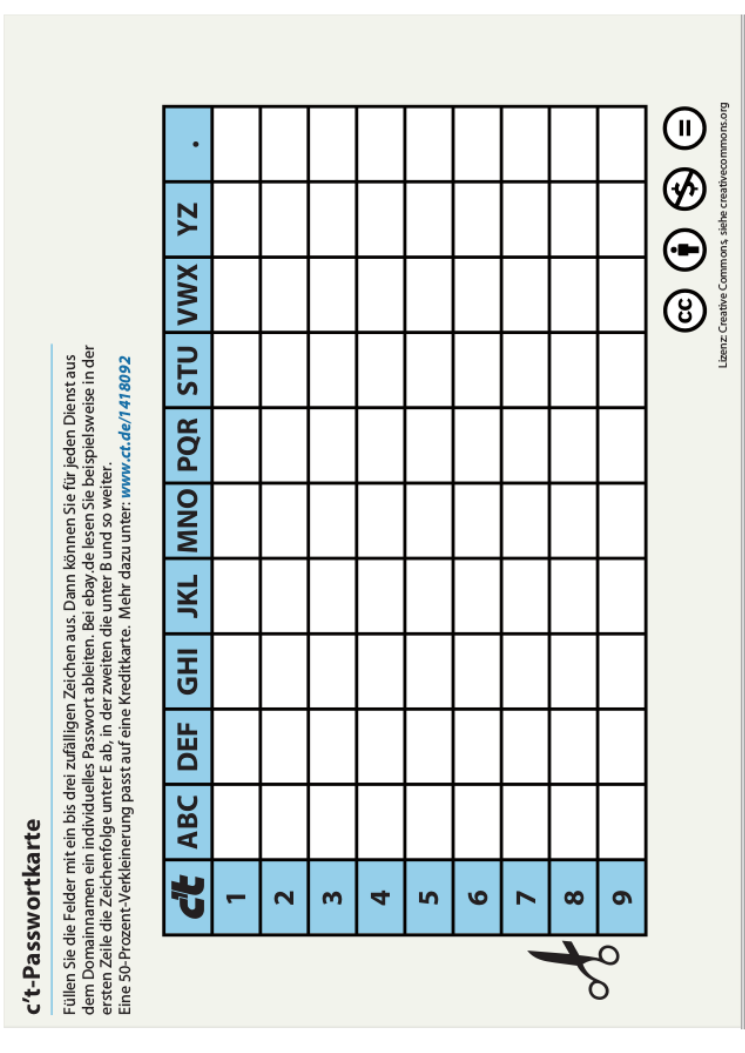
\includegraphics[width=0.5\textwidth, angle=270]{Bilder/CTpasswort.png}
    \end{center}
\end{frame}

%FIXME: Weiß gerade nicht, ob dies der beste Ort für diesen Inhalt ist.
% Vllt. besser zwischen "So schnell knackbar" und den Merkmethoden
%FIXME: Mag den Folientitel noch nicht.
\begin{frame}{Noch ein paar Hinweise}
    \begin{alertblock}{Immer neue Passwörter}
        %alt: Es ist zwar nervig, aber jeder Dienst braucht ein eigenes neues Passwort!
        %neu:\Wendy{
        Jeder Dienst braucht ein eigenes, neues Passwort - nervig, aber sicherer!%}
    \end{alertblock}

    \pause\begin{alertblock}{Wie vertrauensvoll ist ein Dienst?}
        Einem Dienst, der euch keine Sonderzeichen und/oder nur stark begrenzte Zeichenanzahl erlaubt, sollten keine wichtige Daten anvertraut werden! \\%\Wendy{konjunktiv, deine Meinung}
        Besser sogar: gar nicht erst benutzen!
    \end{alertblock}
\end{frame}
\section{Autentifizierungs Alternativen}
\begin{frame}{SmartCard}
    \begin{center}
        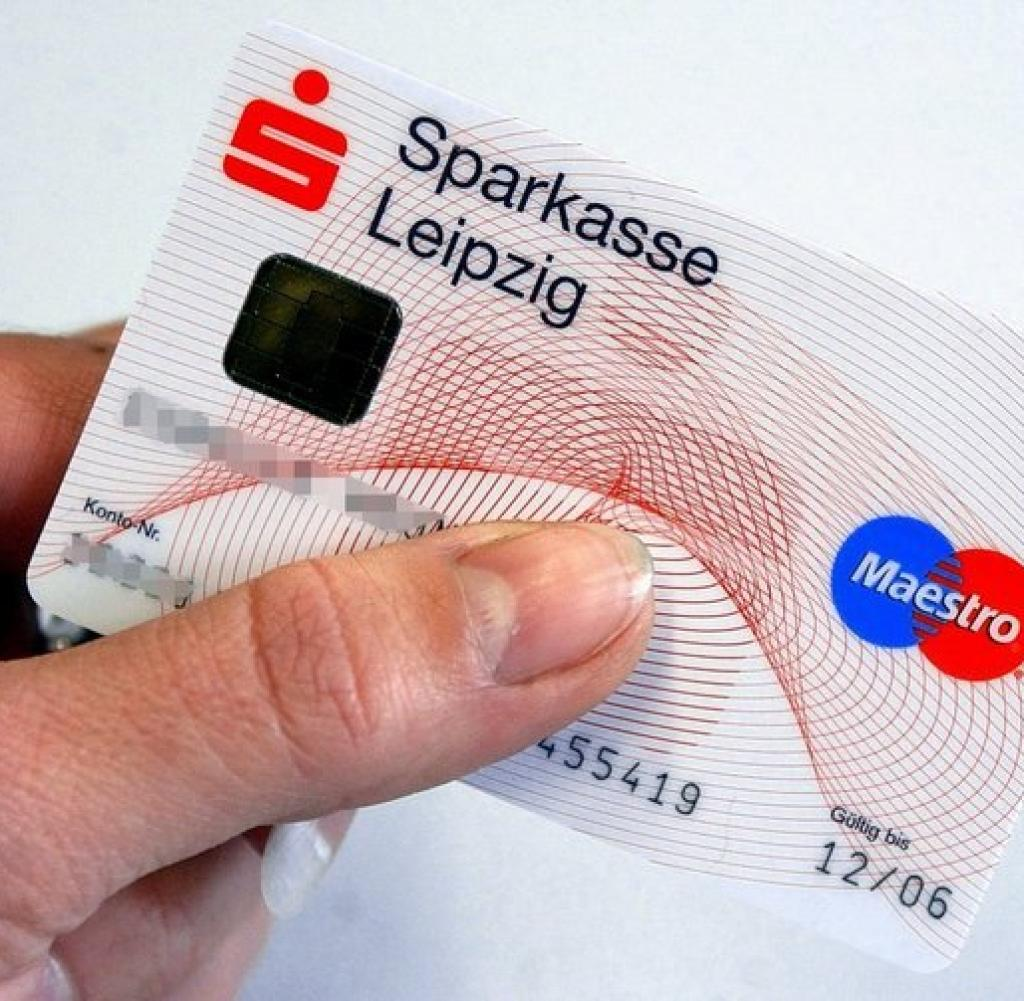
\includegraphics[width=0.5\textwidth]{Bilder/EC.jpg}
    \end{center}
\end{frame}
\begin{frame}{EC Karte}
Die EC Karte ist ein Gutes Beispiel für Zwei Faktor Authentifizierung und SmartCard.\\
Der Chip beinhaltet verschlüssete Informationen die den Kunden Idetifizieren, zusätzlich muss der Kunde ein Pin zu Bezahlung eingeben.\\
\ \\
\textbf{Nur die Kombination gibt die Freigabe für die Zahlung}\\
(Ja es gibt inzwichen einschränkungen)
\end{frame}
\begin{frame}{2Faktor}
Bei der zwei Faktor Authentifizierung ist das Wichtige das es eine Zweite Prüfung deiner Autentität beweist.\\
\begin{itemize}
\item SMS
\item SmartCard
\item Token Generatoren
\end{itemize}
\end{frame}
\begin{frame}{GPG Karten Falls noch Zeit ist}

\end{frame}
\end{document}
